%% paper_template.tex is a modification of:
%% bare_conf.tex 
%% V1.2
%% 2002/11/18
%% by Michael Shell
%% mshell@ece.gatech.edu
%% 
%% This is a skeleton file demonstrating the use of IEEEtran.cls 
%% (requires IEEEtran.cls version 1.6b or later) with an IEEE conference paper.
%% 
%% Support sites:
%% http://www.ieee.org
%% and/or
%% http://www.ctan.org/tex-archive/macros/latex/contrib/supported/IEEEtran/ 
%%
%% This code is offered as-is - no warranty - user assumes all risk.
%% Free to use, distribute and modify.

% *** Authors should verify (and, if needed, correct) their LaTeX system  ***
% *** with the testflow diagnostic prior to trusting their LaTeX platform ***
% *** with production work. IEEE's font choices can trigger bugs that do  ***
% *** not appear when using other class files.                            ***
% Testflow can be obtained at:
% http://www.ctan.org/tex-archive/macros/latex/contrib/supported/IEEEtran/testflow


% Note that the a4paper option is mainly intended so that authors in
% countries using A4 can easily print to A4 and see how their papers will
% look in print. Authors are encouraged to use U.S. letter paper when 
% submitting to IEEE. Use the testflow package mentioned above to verify
% correct handling of both paper sizes by the author's LaTeX system.
%
% Also note that the "draftcls" or "draftclsnofoot", not "draft", option
% should be used if it is desired that the figures are to be displayed in
% draft mode.
%
% This paper can be formatted using the % (instead of conference) mode.
%++++++++++++++++++++++++++++++++++++++++++++++++++++++
%\documentclass[conference]{IEEEims} % Modified for MTT-IMS
%\documentclass[conference]{IMSTemplate}
\documentclass[conference]{IEEEtran}
%++++++++++++++++++++++++++++++++++++++++++++++++++++++
% If the IEEEtran.cls has not been installed into the LaTeX system files, 
% manually specify the path to it:
% \documentclass[conference]{../sty/IEEEtran} 


% some very useful LaTeX packages include:

%\usepackage{cite}      % Written by Donald Arseneau
                        % V1.6 and later of IEEEtran pre-defines the format
                        % of the cite.sty package \cite{} output to follow
                        % that of IEEE. Loading the cite package will
                        % result in citation numbers being automatically
                        % sorted and properly "ranged". i.e.,
                        % [1], [9], [2], [7], [5], [6]
                        % (without using cite.sty)
                        % will become:
                        % [1], [2], [5]--[7], [9] (using cite.sty)
                        % cite.sty's \cite will automatically add leading
                        % space, if needed. Use cite.sty's noadjust option
                        % (cite.sty V3.8 and later) if you want to turn this
                        % off. cite.sty is already installed on most LaTeX
                        % systems. The latest version can be obtained at:
                        % http://www.ctan.org/tex-archive/macros/latex/contrib/supported/cite/

%\usepackage{graphicx}  % Written by David Carlisle and Sebastian Rahtz
                        % Required if you want graphics, photos, etc.
                        % graphicx.sty is already installed on most LaTeX
                        % systems. The latest version and documentation can
                        % be obtained at:
                        % http://www.ctan.org/tex-archive/macros/latex/required/graphics/
                        % Another good source of documentation is "Using
                        % Imported Graphics in LaTeX2e" by Keith Reckdahl
                        % which can be found as esplatex.ps and epslatex.pdf
                        % at: http://www.ctan.org/tex-archive/info/
% NOTE: for dual use with latex and pdflatex, instead load graphicx like:
%\ifx\pdfoutput\undefined
%\usepackage{graphicx}
%\else
%\usepackage[pdftex]{graphicx}
%\fi
%+++++++++++++++++++++++++++++++++++++++++++
% Added to commands
\input epsf
\usepackage{graphicx}

%+++++++++++++++++++++++++++++++++++++++++++
% However, be warned that pdflatex will require graphics to be in PDF
% (not EPS) format and will preclude the use of PostScript based LaTeX
% packages such as psfrag.sty and pstricks.sty. IEEE conferences typically
% allow PDF graphics (and hence pdfLaTeX). However, IEEE journals do not
% (yet) allow image formats other than EPS or TIFF. Therefore, authors of
% journal papers should use traditional LaTeX with EPS graphics.
%
% The path(s) to the graphics files can also be declared: e.g.,
% \graphicspath{{../eps/}{../ps/}}
% if the graphics files are not located in the same directory as the
% .tex file. This can be done in each branch of the conditional above
% (after graphicx is loaded) to handle the EPS and PDF cases separately.
% In this way, full path information will not have to be specified in
% each \includegraphics command.
%
% Note that, when switching from latex to pdflatex and vice-versa, the new
% compiler will have to be run twice to clear some warnings.


%\usepackage{psfrag}    % Written by Craig Barratt, Michael C. Grant,
                        % and David Carlisle
                        % This package allows you to substitute LaTeX
                        % commands for text in imported EPS graphic files.
                        % In this way, LaTeX symbols can be placed into
                        % graphics that have been generated by other
                        % applications. You must use latex->dvips->ps2pdf
                        % workflow (not direct pdf output from pdflatex) if
                        % you wish to use this capability because it works
                        % via some PostScript tricks. Alternatively, the
                        % graphics could be processed as separate files via
                        % psfrag and dvips, then converted to PDF for
                        % inclusion in the main file which uses pdflatex.
                        % Docs are in "The PSfrag System" by Michael C. Grant
                        % and David Carlisle. There is also some information 
                        % about using psfrag in "Using Imported Graphics in
                        % LaTeX2e" by Keith Reckdahl which documents the
                        % graphicx package (see above). The psfrag package
                        % and documentation can be obtained at:
                        % http://www.ctan.org/tex-archive/macros/latex/contrib/supported/psfrag/

%\usepackage{subfigure} % Written by Steven Douglas Cochran
                        % This package makes it easy to put subfigures
                        % in your figures. i.e., "figure 1a and 1b"
                        % Docs are in "Using Imported Graphics in LaTeX2e"
                        % by Keith Reckdahl which also documents the graphicx
                        % package (see above). subfigure.sty is already
                        % installed on most LaTeX systems. The latest version
                        % and documentation can be obtained at:
                        % http://www.ctan.org/tex-archive/macros/latex/contrib/supported/subfigure/

%\usepackage{url}       % Written by Donald Arseneau
                        % Provides better support for handling and breaking
                        % URLs. url.sty is already installed on most LaTeX
                        % systems. The latest version can be obtained at:
                        % http://www.ctan.org/tex-archive/macros/latex/contrib/other/misc/
                        % Read the url.sty source comments for usage information.

%\usepackage{stfloats}  % Written by Sigitas Tolusis
                        % Gives LaTeX2e the ability to do double column
                        % floats at the bottom of the page as well as the top.
                        % (e.g., "\begin{figure*}[!b]" is not normally
                        % possible in LaTeX2e). This is an invasive package
                        % which rewrites many portions of the LaTeX2e output
                        % routines. It may not work with other packages that
                        % modify the LaTeX2e output routine and/or with other
                        % versions of LaTeX. The latest version and
                        % documentation can be obtained at:
                        % http://www.ctan.org/tex-archive/macros/latex/contrib/supported/sttools/
                        % Documentation is contained in the stfloats.sty
                        % comments as well as in the presfull.pdf file.
                        % Do not use the stfloats baselinefloat ability as
                        % IEEE does not allow \baselineskip to stretch.
                        % Authors submitting work to the IEEE should note
                        % that IEEE rarely uses double column equations and
                        % that authors should try to avoid such use.
                        % Do not be tempted to use the cuted.sty or
                        % midfloat.sty package (by the same author) as IEEE
                        % does not format its papers in such ways.

%\usepackage{amsmath}   % From the American Mathematical Society
                        % A popular package that provides many helpful commands
                        % for dealing with mathematics. Note that the AMSmath
                        % package sets \interdisplaylinepenalty to 10000 thus
                        % preventing page breaks from occurring within multiline
                        % equations. Use:
%\interdisplaylinepenalty=2500
                        % after loading amsmath to restore such page breaks
                        % as IEEEtran.cls normally does. amsmath.sty is already
                        % installed on most LaTeX systems. The latest version
                        % and documentation can be obtained at:
                        % http://www.ctan.org/tex-archive/macros/latex/required/amslatex/math/



% Other popular packages for formatting tables and equations include:

%\usepackage{array}
% Frank Mittelbach's and David Carlisle's array.sty which improves the
% LaTeX2e array and tabular environments to provide better appearances and
% additional user controls. array.sty is already installed on most systems.
% The latest version and documentation can be obtained at:
% http://www.ctan.org/tex-archive/macros/latex/required/tools/

% Mark Wooding's extremely powerful MDW tools, especially mdwmath.sty and
% mdwtab.sty which are used to format equations and tables, respectively.
% The MDWtools set is already installed on most LaTeX systems. The lastest
% version and documentation is available at:
% http://www.ctan.org/tex-archive/macros/latex/contrib/supported/mdwtools/


% V1.6 of IEEEtran contains the IEEEeqnarray family of commands that can
% be used to generate multiline equations as well as matrices, tables, etc.


% Also of notable interest:

% Scott Pakin's eqparbox package for creating (automatically sized) equal
% width boxes. Available:
% http://www.ctan.org/tex-archive/macros/latex/contrib/supported/eqparbox/



% Notes on hyperref:
% IEEEtran.cls attempts to be compliant with the hyperref package, written
% by Heiko Oberdiek and Sebastian Rahtz, which provides hyperlinks within
% a document as well as an index for PDF files (produced via pdflatex).
% However, it is a tad difficult to properly interface LaTeX classes and
% packages with this (necessarily) complex and invasive package. It is
% recommended that hyperref not be used for work that is to be submitted
% to the IEEE. Users who wish to use hyperref *must* ensure that their
% hyperref version is 6.72u or later *and* IEEEtran.cls is version 1.6b 
% or later. The latest version of hyperref can be obtained at:
%
% http://www.ctan.org/tex-archive/macros/latex/contrib/supported/hyperref/
%
% Also, be aware that cite.sty (as of version 3.9, 11/2001) and hyperref.sty
% (as of version 6.72t, 2002/07/25) do not work optimally together.
% To mediate the differences between these two packages, IEEEtran.cls, as
% of v1.6b, predefines a command that fools hyperref into thinking that
% the natbib package is being used - causing it not to modify the existing
% citation commands, and allowing cite.sty to operate as normal. However,
% as a result, citation numbers will not be hyperlinked. Another side effect
% of this approach is that the natbib.sty package will not properly load
% under IEEEtran.cls. However, current versions of natbib are not capable
% of compressing and sorting citation numbers in IEEE's style - so this
% should not be an issue. If, for some strange reason, the user wants to
% load natbib.sty under IEEEtran.cls, the following code must be placed
% before natbib.sty can be loaded:
%
% \makeatletter
% \let\NAT@parse\undefined
% \makeatother
%
% Hyperref should be loaded differently depending on whether pdflatex
% or traditional latex is being used:
%
%\ifx\pdfoutput\undefined
%\usepackage[hypertex]{hyperref}
%\else
%\usepackage[pdftex,hypertexnames=false]{hyperref}
%\fi
%
% Pdflatex produces superior hyperref results and is the recommended
% compiler for such use.



% *** Do not adjust lengths that control margins, column widths, etc. ***
% *** Do not use packages that alter fonts (such as pslatex).         ***
% There should be no need to do such things with IEEEtran.cls V1.6 and later.


% correct bad hyphenation here
\hyphenation{op-tical net-works semi-conduc-tor IEEEtran}
\begin{document}

% paper title
%\title{Submission Format for IMS2014 (Title in 24-point Times font)}
% If the \LARGE is deleted, the title font defaults to  24-point.
% Actually, 
% the \LARGE sets the title at 17 pt, which is close enough to 18-point.
%+++++++++++++++++++++++++++++++++++++++++++
\title{\LARGE Decentralized Machine Learning Models with Cryptography Algorithms}
%+++++++++++++++++++++++++++++++++++++++++++
% author names and affiliations
% use a multiple column layout for up to three different
% affiliations
%+++++++++++++++++++++++++++++++++++++++++++
%\author{\authorblockN{J. Clerk Maxwell}
%\authorblockA{School of Electrical and\\Computer Engineering\\
%Somewhere Institute of Technology\\
%City, State 54321--0000\\
%Email: maxwell@curl.edu}
%\and
%\authorblockN{Michael Faraday}
%\authorblockA{(List authors on this line using 12 point Times font\\ - use a second line if necessary)\\
%Microwave Research\\
%City, State/Region, Mail/Zip Code, Country\\
%Email: homer@thesimpsons.com}
%\and
%\authorblockN{Andr\'e M. Amp\`ere \\ }
%\authorblockA{Starfleet Academy\\
%San Francisco, CA 96678-2391\\
%Telephone: (800) 555--1212\\
%Fax: (888) 555--1212}}

\author{\authorblockN{Aman, Prof. Siba Narayan Swain, Prof. Mahadeva Prasanna}
\authorblockA{\authorrefmark{1}BTP Autumn Semester 2020 Report}}


%+++++++++++++++++++++++++++++++++++++++++++++++++++

% avoiding spaces at the end of the author lines is not a problem with
% conference papers because we don't use \thanks or \IEEEmembership


% for over three affiliations, or if they all won't fit within the width
% of the page, use this alternative format:
% 
% Another example.
%\author{\authorblockN{Michael Shell\authorrefmark{1},
%Homer Simpson\authorrefmark{2},
%James Kirk\authorrefmark{3}, 
%Montgomery Scott\authorrefmark{3} and
%Eldon Tyrell\authorrefmark{4}}
%\authorblockA{\authorrefmark{1}School of Electrical and Computer Engineering\\
%Georgia Institute of Technology,
%Atlanta, Georgia 30332--0250\\ Email: mshell@ece.gatech.edu}
%\authorblockA{\authorrefmark{2}Twentieth Century Fox, Springfield, USA\\
%Email: homer@thesimpsons.com}
%\authorblockA{\authorrefmark{3}Starfleet Academy, San Francisco, California 96678-2391\\
%Telephone: (800) 555--1212, Fax: (888) 555--1212}
%\authorblockA{\authorrefmark{4}Tyrell Inc., 123 Replicant Street, Los Angeles, California 90210--4321}}



% use only for invited papers
%\specialpapernotice{(Invited Paper)}

% make the title area
\maketitle

\begin{abstract}
Machine learning models trained on sensitive real-world data promise improvements to everything from medical screening to disease outbreak discovery. And the widespread use of mobile devices means even richer—and more sensitive—data is becoming available. However, Traditional machine learning involves a data pipeline that uses a central server(on-prem or cloud) that hosts the trained model in order to make predictions. Distributed Machine Learning (FL) in contrast, is an approach that downloads the current model and computes an updated model at the device itself (a.k.a edge computing) using local data. These locally trained models are then sent from the devices back to the central server where they are aggregated, i.e. averaging weights, and then a single consolidated and improved global model is sent back to the devices. However, parameter interaction and the resulting model still might disclose information about the training
data used. To address these privacy concerns, two approaches have been used based in this report which is based on Homographic Encryption and Secret Sharing technique among others. The report summarizes the research done in these areas and provides suggestions for future directions in research.

\end{abstract}

\vspace{\baselineskip} 

\IEEEoverridecommandlockouts
\begin{keywords}
Cryptography, Neural Network, Privacy-preserving, Homographic Encryption, Secret Sharing Scheme.
\end{keywords}
% no keywords

% For peer review papers, you can put extra information on the cover
% page as needed:
% \begin{center} \bfseries EDICS Category: 3-BBND \end{center}
%
% for peerreview papers, inserts a page break and creates the second title.
% Will be ignored for other modes.
\IEEEpeerreviewmaketitle



\section{Introduction}
% no \PARstart
Advancements in machine learning algorithms have resulted in a widespread adoption across industries. Nonetheless, areas dealing with sensitive and private data, like healthcare or finance, have lagged behind due to regulatory constraints to protect users’ data.
With the emergence of Machine Learning as a Service, entities are providing model inference as a service. We can distinguish three parties in such scenarios, a model owner such as a hospital who has trained a model, a host such as a cloud provider providing computing power, and a client wanting to benefit from the service. A model owner can also be a host in some scenarios. Trust must be established between those parties as the client does not want her data to be leaked, and the model owner wants to protect her model. However, large-scale collection of sensitive data entails risks. At the same time, with the increasing awareness of large companies compromising on data security and user privacy, the emphasis on data privacy and security has become a worldwide
major issue. News about leaks on public data are causing great concerns in public media and
governments. This work outlines an approach to advancing privacy-preserving machine learning by leveraging secure multiparty computation (MPC) to compute sums of model parameter updates from individual users’ devices in a secure manner. The problem of computing a multiparty sum where no party reveals its update in the clear—even to the aggregator—is referred to as Secure Aggregation. The secure aggregation primitive can be used to privately combine the outputs of local machine learning on user devices, in order to update a global model. Training models in this way offers tangible benefits—a user’s device can share an update knowing that the service provider will only see that update after it has been averaged with those of other users. The secure aggregation problem has been a rich area of research: different approaches include works based on generic secure multi-party computation protocols, works based on DC-nets, works based on partially- or fully-homographic threshold encryption, and works based on pairwise masking. We discuss these existing works in more detail in Section 9, and compare them to our approach. 
Mutual research of machine learning and cryptography is not a new area. In addition to cryptography and machine learning has a wide range of applications in relation to information and network security. A none-exhaustive list of examples can be found here:- 

\vspace{\baselineskip} 

\begin{enumerate} 
 \setlength{\itemsep}{-2ex}  
 \setlength{\parskip}{0ex} 
 \setlength{\parsep}{0ex}
\item Network anomaly detection\hfil\break
\item Malware analysis and detection.\hfil\break
\item Homomorphic encrpytion applications \hfil\break
\item Attacks on Physical Unclonable Functions\hfil\break
\item Using machine learning to develop Intrusion Detection System (IDS)\hfil\break
\item Malicious code classification and identification
\end{enumerate}

\vspace{\baselineskip} 

To address the aforementioned security concerns, and considering the universality nature of neural networks, we explore integration of neural networks with cryptography's techniques to design a secure Decentralized learning system with a semi-honest(curious to know) server. Specifically, we design a secure decentralized based general learning system by transferring encrypted weights over distributed system, which consists of initialization, local weight computation, and global weight aggregation.
We are particularly focused on the setting of mobile devices, where communication is extremely expensive, and dropouts are common. Given these constraints, we would like to discuss two popular cryptography techniques i.e. Homographic Encryption, Secret Sharing in a distributed machine learning system and compare the two approaches in terms of loss and performance.
% \begin{table*}
% \centerline { TABLE 1  } 
% \vskip5pt
% \centerline { Summary of Typographical Settings}
% \vskip2pt
% \centerline{
% \vbox{\offinterlineskip
% \hrule
% %\vskip2pt\hrule\vskip2pt
% % Leading & means preamble template repeats infinitely. p.241 TeX Book.
% \halign{&\vrule#&
% \strut\quad#\hfil\quad\cr
% %Use either first and third lines following this description, OR the
% %second line.  The first choice is used when all vertical rules go to the
% %top of the first horizontal line of the table.  The second choice below
% %(with the \strut) is used when there are column headings that span
% %more than one column.  The \strut in that column line will not have the
% %vertical tic marks in the horizontal rule.  Note that a vrule is also
% %considered a column, so when using \multispanx, x is the number of
% %all columns including the ``vrule.'' 
% %height2pt&\omit&&\omit&&\omit&&\omit&&\omit&&\omit&&\omit&&\omit&&\omit&\cr
% &\strut &&\multispan5\hfil {\bf Font Specifics}\hfil&&\multispan9\hfil {\bf Paragraph Description}\hfil &\cr
% %&\omit &&\multispan5\hfil {\bf Font Specifics}\hfil&&\multispan9\hfil {\bf Paragraph Description}\hfil &\cr
% &{\bf Section}&&\multispan5\hfil (Times Roman unless
% specified)\hfil&&\multispan5\hfil spacing (in points)\hfil &&
% alignment&&indent&\cr
% &\omit&&style&&size&&special&&line&&before&&after&&\omit&&(in inches)&\cr
% height2pt&\omit&&\omit&&\omit&&\omit&&\omit&&\omit&&\omit&&\omit&&\omit&\cr
% \noalign{\hrule}
% height2pt&\omit&&\omit&&\omit&&\omit&&\omit&&\omit&&\omit&&\omit&&\omit&\cr
% %\noalign{\vskip2pt\hrule\vskip2pt}
% %\omit&\omit&\omit&\omit\cr
% &Title&&plain&&18&&none&&single&&6&&6&&centered&&none&\cr
% &Autohr List&&plain&&12&&mpme&&single&&6&&6&&centered&&none&\cr
% &Affiliations&&plain&&12&&none&&single&&6&&6&&centered&&none&\cr
% &Abstract&&bold&&9&&none&&exactly 10&&0&&0&&justified&&0.125 $1^{st}$ line&\cr
% &Headings&&plain&&10&&small caps&&exactly 12&&18&&6&&centered&&none&\cr
% &Subheadings&&italic&&10&&none&&exactly 12&&6&&6&&left&&none&\cr
% &Body&&plain&&10&&none&&exactly 12&&0&&0&&justified&&0.125 $1^{st}$ line&\cr
% &Paragrahps&&\omit&&\omit&&\omit&&\omit&&\omit&&\omit&&\omit&&\omit&\cr
% &Equations&&\multispan5 \hfil Symbol font for special characters
% \hfil&&single&&6&&6&&centered&&none&\cr
% &Figures&&\multispan5 \hfil 6 to 9 point sans serif (Helvetica)\hfil&&single&&0&&0&&centered&&none&\cr
% &Figure Captions&&plain&&9&&none &&10&&0&&0&&justified&&none, tab at 0.5&\cr
% &References&&plain&&9&&none&&10&&0&&0&&justified&&0.25 hanging&\cr
% height2pt&\omit&&\omit&&\omit&&\omit&&\omit&&\omit&&\omit&&\omit&&\omit&\cr}
% \hrule}}
% \end{table*}
\section{Background}
In this section, we introduce the background and explain the underlying building blocks i.e. {\itshape Federated Learning}, {\itshape Homographic Encryption} and {\itshape Secret Sharing} of our proposed framework in Figure 1.

\begin{figure}
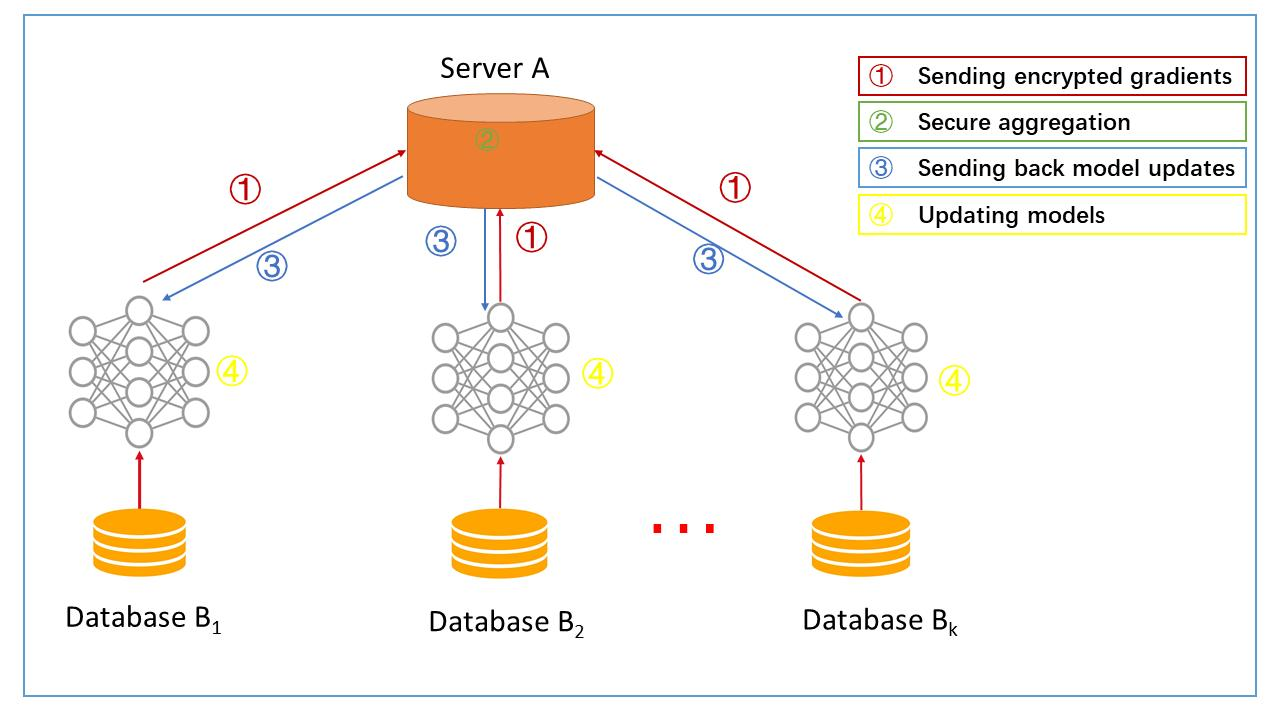
\includegraphics[width=90mm,scale=0.7]{fig.jpg}
%\epsfxsize=3.25in\epsfbox{figure1.epsi}
\caption{ Architecture of Distributed Machine Learning system and overview of how an iteration  works during general federated learning model.}

\vspace{\baselineskip}

\subsection{Federated Learning}\label{AA}
Google has built one of the most secure and robust cloud infrastructures for processing the data to make our services better. Now for models trained from user interaction with mobile devices, we're discussing an additional approach: Federated Learning.
Federated Learning (FL) is an approach that downloads the current model and computes an updated model at the device itself (a.k.a edge computing) using local data. These locally trained models are then sent from the devices back to the central server where they are aggregated, i.e. averaging weights, and then a single consolidated and improved global model is sent back to the devices.
\end{figure}
Federated Learning enables mobile phones to collaboratively learn a shared prediction model while keeping all the training data on device, decoupling the ability to do machine learning from the need to store the data in the cloud. This goes beyond the use of local models that make predictions on mobile devices (like the Mobile Vision API and On-Device Smart Reply) by bringing model training to the device as well.

\begin{figure} 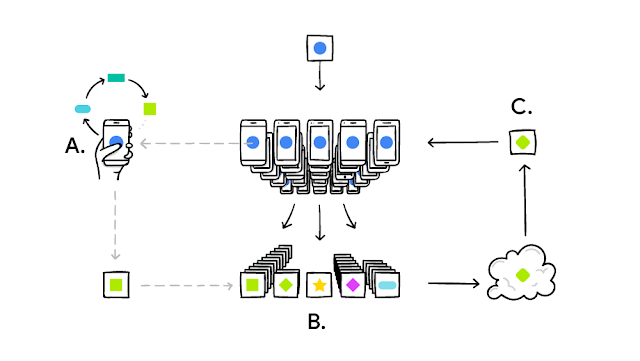
\includegraphics[width=90mm,scale=0.7]{2.png}\caption{Your phone personalizes the model locally, based on your usage (A). Many users' updates are aggregated (B) to form a consensus change (C) to the shared model, after which the procedure is repeated}
\end{figure}

Federated Learning allows for smarter models, lower latency, and less power consumption, all while ensuring privacy. 

Given a secret {\itshape S}, we would like n parties to share the secret so that the following properties hold:

\begin{enumerate} 
 \setlength{\itemsep}{-2ex}  
 \setlength{\parskip}{0ex} 
 \setlength{\parsep}{0ex}
\item All {\itshape N} parties can get together and recover {\itshape S} \hfil\break
\item Less than n parties cannot recover {\itshape S} \hfil\break
\end{enumerate}

As shown in the figure 3, we have a secret {\itshape x} which is distributed among all shrareholders {\itshape x1, x2, x3 ... xn} and reconstructed as secret {\itshape x} after the aggregation.
\begin{figure}

And this approach has another immediate benefit: in addition to providing an update to the shared model, the improved model on your phone can also be used immediately, powering experiences personalized by the way you use your phone.

\subsection{Homographic Encryption}
Homographic Encryption is a public key cryptographic scheme. The user creates a pair of secret and public key, uses the public one to encrypt her data, before sending it to a third party which will perform computations on the encrypted data. Because of the homomorphic properties of the encryption and decryption, the user can get the encrypted result and decode it with her own key to see the output of the computation on her data, without having shown it once in clear to the third party.
It admits some kind of computations on encrypted data. In particular, given an input x encrypted as  {\itshape Enc(x)}, it should be possible to publicly compute {\itshape Enc(x)} for a function f taken from some class of functions. The key point here is “publicly”, meaning that carrying out this computation has to be possible without having access to any secret information

\vspace{\baselineskip}

\subsection{ Secret Sharing }

In cryptography, secret sharing refers to any method for distributing a secret among a group of participants, each of which allocates a share of the secret. The secret can only be reconstructed when the shares are combined together; individual shares are of no use on their own.

\vspace{\baselineskip}
\vspace{\baselineskip}

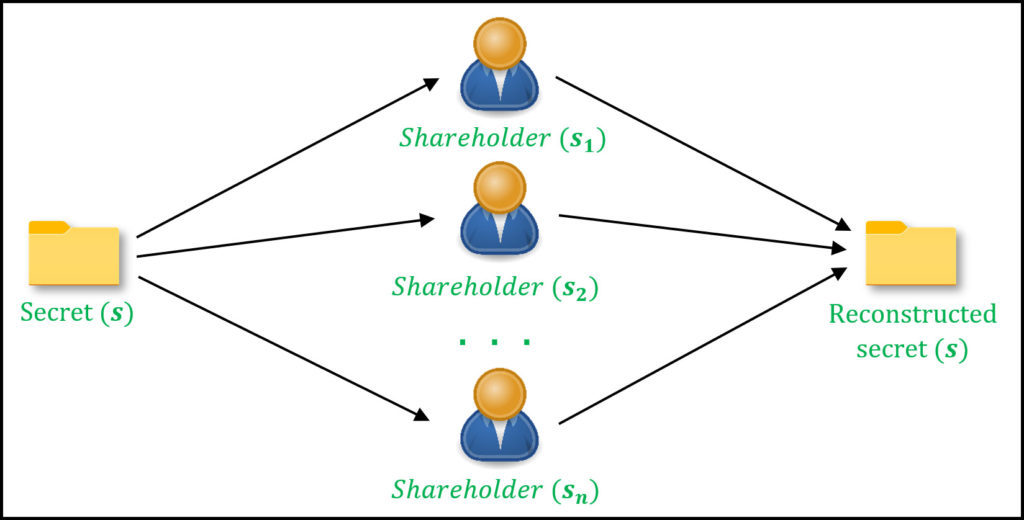
\includegraphics[width=90mm,scale=0.7]{12.jpg}
%\epsfxsize=3.25in\epsfbox{figure1.epsi}
\caption{Secret sharing (also called secret splitting) which refers to methods for distributing a secret among a group of participants, each of whom is allocated a share of the secret is shown in the figure. }
\end{figure}

\vspace{\baselineskip}

 \setlength{\itemsep}{-2ex}  
 \setlength{\parskip}{0ex} 
 \setlength{\parsep}{0ex}

\begin{figure}

\section{Problem Formulation}
In this section, we mathematically formulate the concept of federated learning and then discuss about the problems related to above approach and various threats to the model i.e. {\itshape Fault Tolerance}, {\itshape Malicious Clients}.

\subsection{Maths behind the Federated Learning}\label{AA}

Initially we will serialize the weights present in between the layers of the neural network of client $C_p$. Let there be $L_1,L_2,...,L_n$ layers, i.e., if $W_1$ is a m*n matrix
\begin{equation}
L_1 = {W_{1,1},W_{1,2},...,W_{1,n},W_{2,1},..,...,W_{m,1},W_{m,2},...W_{m,n}} 
\end{equation}
Similarly, for other layers, we will serialize $L_2,L_3,...,L_n$ 
and make a vector 
\begin{equation}
    L^{k} = {L_1,L_2,...,L_k}
\end{equation}
representing serialized weights from client $C_p$.

Now at the server we aggregate the layers from different clients
\begin{equation}
    L_{avg} = \frac{1}{P} \sum_{p=1}^{P} L_{p}
\end{equation}
    where P number of clients send weights to the server.

\vspace{\baselineskip}

\textbf{Privacy Leak}: An Issue Caused by insecure communication where the privacy of the shared parameters of the clients can be leaked and server can also learn about the shared weights or parameters. Given that the model’s parameters are trained based on the user’s data, there is a chance of getting information about the data from such parameters. The updates transmitted from the device to the server should be minimal. There’s no need to share more than the minimum amount of info required to update the model at the server. Otherwise, there remains the possibility of private data being exposed and intercepted. The private data is this vulnerable, even without being sent explicitly to the server because it’s possible to restore it based on the parameters trained by such data. In the worst case when an attacker is able to restore the data, it should be anonymous as much as possible without revealing some user’s private information like the name for example.

\vspace{\baselineskip}


\textbf{Data Poisoning}: In FL, clients, who previously acted only as passive data providers, can now observe intermediate model states and might contribute arbitrary updates as part of the decentralized training process. This creates an opportunity for malicious
clients to manipulate the training process with little restriction.

\vspace{\baselineskip}

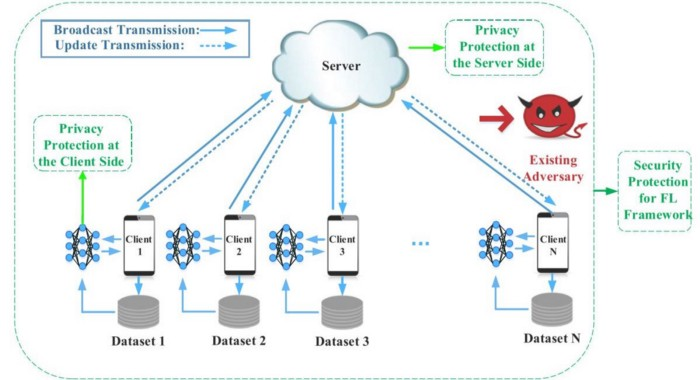
\includegraphics[width=90mm,scale=0.7]{14.jpeg}
%\epsfxsize=3.25in\epsfbox{figure1.epsi}
\caption{Malicious client responsible for data poisoning.}
\end{figure}

\vspace{\baselineskip}

\begin{figure}

\textbf{Model Aggregation Issue}: The aggregation is mainly processed at the server after
collecting individuals’ parameters, and updates the global model. This process is particularly important as it should absorb the advantages of the clients and determine the end of learning. If protection method is applied at the client side, such as the perturbation applied before collecting model parameters, the aggregation cannot be simply a conventional averaging
process. The main reasons can be concluded as: (i) the noise power of perturbation is increasing along with the number of clients; (ii) the server should know the stochastic information from clients and the design of the aggregation method needs to distinguish the privacy-sensitive clients from privacy insensitive ones.

\vspace{\baselineskip}

% \begin{eqnarray}
% \oint {\bf E \cdot dL} & = & - {\partial\over \partial t}
% \int\!\!\!\int {\bf B \cdot} d {\bf S}\\
% \noalign{\hbox{or}}
% \nabla \times {\bf H} & = & {\bf J} + {\partial {\bf D} \over \partial t}.
% \end{eqnarray}

\section{Experimental Results and Possible Solutions}
In this section, we discuss about the possible solutions and some experimental results to solve the above problems.

\subsection{Homographic Encryption with Authentication for privacy leak }
As discussed in Section 2, After the client trains the model by its private data, the model is sent to the server. At this time, an attacker might hack some of the Apis of the model to make it behave for their benefit. For example, the attacker might control the labels assigned to images with certain features. As for the security of the whole FL framework, it mainly considers the model stealing attacks. Specially, any participant in FL may introduce hidden functionality into the joint global model, e.g., to ensure that an image classifier assigns an attacker-chosen label to images with certain features, or that a word predictor completes certain sentences with an attacker. Consequently, there are also some protecting measures on the security design for FL.
To handle these issues, we used Homographic Encryption with Authentication such that even after sharing the parameters to server or to any other client, it can't be decrypted and the privacy of each of the client is maintained.

\vspace{\baselineskip}

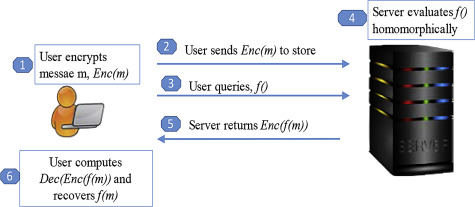
\includegraphics[width=90mm,scale=0.7]{15.jpg}
%\epsfxsize=3.25in\epsfbox{figure1.epsi}

\caption{ Homographically Encrypted Training.}

\vspace{\baselineskip}

\textbf{Homomorphic encryption [12] is adopted to protect user data through parameters exchange under encryption mechanism. That is the parameters are coded before uploading, and the public-private decoding keys are also need to transmit, which cause extra communication cost.}

\vspace{\baselineskip}
\vspace{\baselineskip}

\textbf{Key Steps of Homographic Encryption:} 

\vspace{\baselineskip}

Let P be the plaintext space, i.e., P = \{0,1\} which consists of 

\end{figure}

\begin{figure}

\vspace{\baselineskip}
 
input message tuple (m1, m2,..mn). Let us represent the Boolean circuit by C and ordinary function notation as C (m1, m2,... mn) to represent the evaluation of the circuit on the message tuple . The general HE is described below:

\vspace{\baselineskip}

\begin{itemize}

\item Gen(1$\lambda$, $\alpha$) is the key generation algorithm that generates output keys triplets, i.e., secret key-pair (sk and pk) along with evaluation key (evk), where $\lambda$ is security parameter and $\alpha$ is auxiliary input, (sk, pk, evk) ← KeyGen()

\vspace{\baselineskip}

\item Enc(pk,m) encrypts a message (m) with the public key (pk) and outputs a ciphertext (c $\epsilon$ C), c ← Encpk(m)

\vspace{\baselineskip}

\item Dec(sk, c) decrypts a ciphertexts with the secret key (sk) and recovers message (m) as the output, m ← Decsk(c)

\vspace{\baselineskip}

\item Eval(evk, C, c1, c1, …, cn) produces evaluation output by taking evk key as input, a circuit C$\epsilon$C and tuple of input ciphertexts, i.e., c1…cn and previous evaluation results, c$∗$ ← Evalevk(evk, C, c1, c2, …cn).

\vspace{\baselineskip}

\end{itemize}

\textbf{Observation and Results:}

\vspace{\baselineskip}

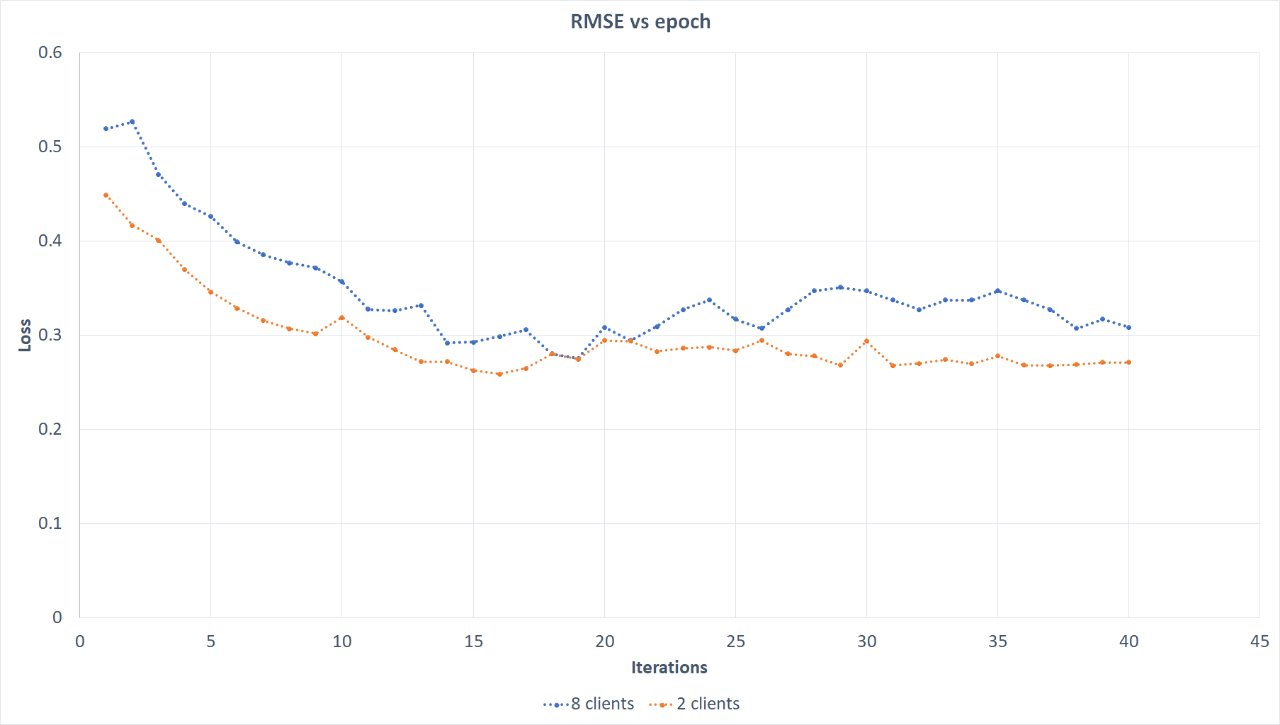
\includegraphics[width=90mm,scale=0.7]{RMSE_HE.jpeg}
%\epsfxsize=3.25in\epsfbox{figure1.epsi}
\caption{ RMSE values variation with number of Iterations in Homographic Encryption for two and eight clients.}

\end{figure}

As shown in the \textbf{figure 6}, we can observe that RMSE values for two clients are decreasing and the model is converging first and then it's almost constant which is expected according to the theoretical aspects. Also, it shows some variation and bumps in case of 8 clients which is happening because of the more data distribution and participation of more clients in aggregation.

\vspace{\baselineskip}

In the \textbf{figure 7}, the wall-clock running time taken by HE algorithm is very large as compared to simple neural network which causes some amount of delay or latency in each iteration w.r.t the neural network without encryption.

\begin{figure}

\vspace{\baselineskip}


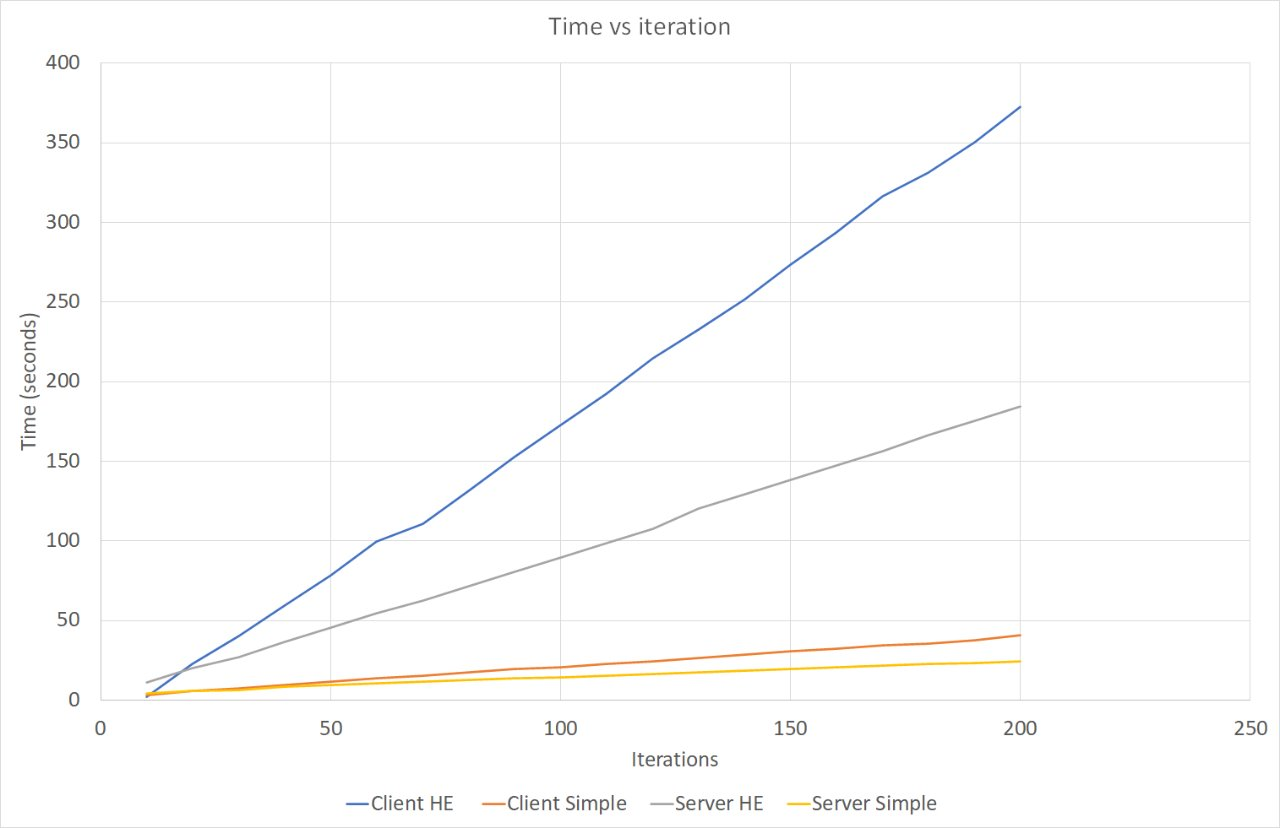
\includegraphics[width=90mm,scale=0.7]{Time_HE.jpeg}
\caption{ Wall-clock running time for the client and server with and without Homographic Encryption in each iteration.}

\end{figure}

\begin{figure}

\vspace{\baselineskip}

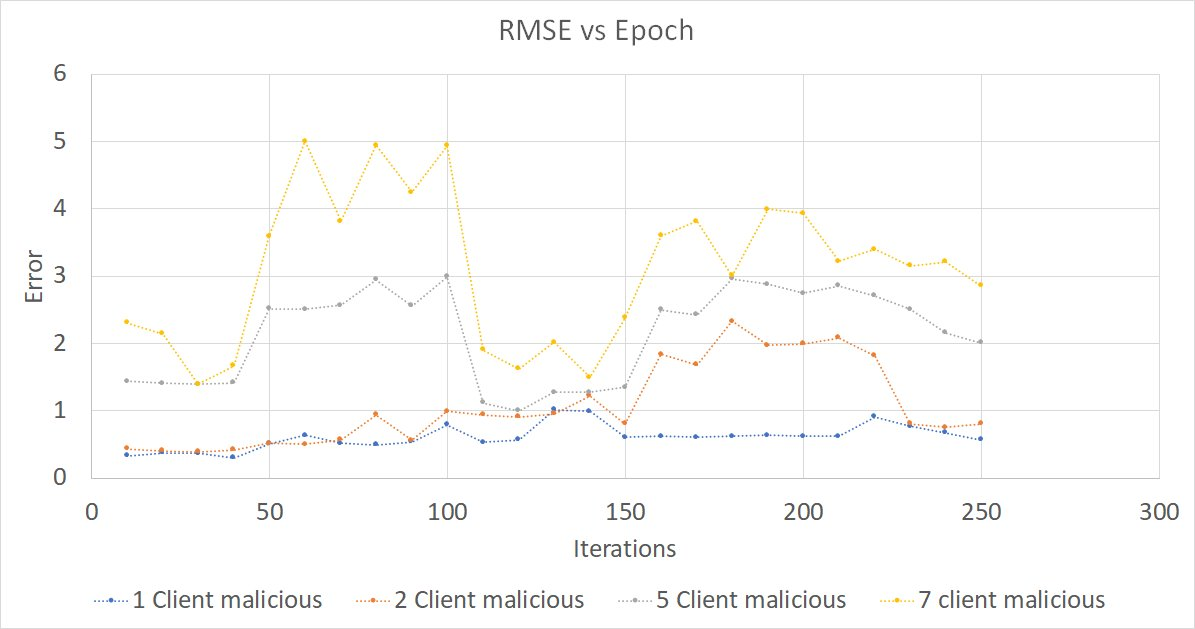
\includegraphics[width=90mm,scale=0.7]{RMSE_Malicious_HE.jpeg}
\caption{ RMSE  values  variation  with  number  of  Iterations for malicious clients}

\vspace{\baselineskip}

we can observe a lot of bumps and variations in RMSE values in \textbf{figure 8} because Homographic Encryption works only for the Semi-honest(curious to know) environment where all the clients and server wants to know each other's parameters but they can't manipulate it. And it's not possible in some scenario. So, we discuss about Secret Sharing technique which can handle all of the above issues to some extent. 

\end{figure}


\subsection{Secret Sharing for reducing Data Poisoning and improving Model Aggregation}
As discussed in section 3, Federated learning (FL) is an emerging paradigm for distributed training of large-scale deep neural networks in which participants’ data remains on their own devices with only model updates being shared with a central server. However, the distributed nature of FL gives rise to new threats caused by potentially malicious participants.
To overcome this issue we see about the secret sharing technique. 
Secret sharing is an old well-known cryptographic primitive, with existing real-world applications in e.g. Bitcoin signatures and password management. But perhaps more interestingly, secret sharing also has strong links to secure computation and may for instance be used for private machine learning. 

\vspace{\baselineskip}

\textbf{The essence of the primitive is that a dealer wants to split a secret into several shares given to shareholders, in such a way that each individual shareholder learns nothing about the secret, yet if sufficiently many re-combine their shares then the secret can be reconstructed. Intuitively, the question of trust changes from being about the integrity of a single individual to the non-collaboration of several parties: it becomes distributed.}

\vspace{\baselineskip}

\textbf{Key Steps of Secret Sharing:} 
The main aim of this algorithm is to divide secret that needs to be encrypted into various unique parts.

\begin{itemize}

\item Let’s say S is the secret that we wish to encode.


\vspace{\baselineskip}

\item It is divided into N parts: S1, S2, S3, …., Sn.

\vspace{\baselineskip}

\item After dividing it, a number K is chosen by the user in order to decrypt the parts and find the original secret.

\vspace{\baselineskip}

\item It is chosen in such a way that if we know less than K parts, then we will not be able to find the secret S (i.e.) the secret S can not be reconstructed with (K – 1) parts or fewer.

\vspace{\baselineskip}

\item If we know K or more parts from S1, S2, S3, …., Sn, then we can compute/reconstructed our secret code S easily. This is conventionally called (K, N) threshold scheme.

\vspace{\baselineskip}

\end{itemize}

\textbf{Approach}: The main idea behind the Secret Sharing Algorithm lies behind the concept that for the given K points we can find a polynomial equation with the degree (K – 1).

\vspace{\baselineskip}

\textbf{Example}:
For the given two points, (x1, y1) and (x2, y2) we can find a linear polynomial ax + by = c.
Similarly, for the given three points, we can find a quadratic polynomial ax2 + bx + cy = d.

So, the idea is to build a polynomial with the degree (K – 1) such that the constant term is the secret code and the remaining numbers are random and this constant term can be found by using any K points out of N points generated from this polynomial by using Lagrange’s Basis Polynomial. 

\vspace{\baselineskip}

Let the secret code S = 65, N = 4, K = 2.

\begin{itemize}

\item Initially, in order to encrypt the secret code, we build a polynomial of degree (K – 1).


\vspace{\baselineskip}

\item Therefore, let the polynomial be y = a + bx. Here, the constant part ‘a’ is our secret code.

\vspace{\baselineskip}

\item Let b be any random number, say b = 15.

\vspace{\baselineskip}

\item Therefore, for this polynomial y = 65 + 15x, we generate N = 4 points from it..

\vspace{\baselineskip}

% \end{itemize}

% \begin{figure}

% \begin{itemize}
\item Let those 4 points be (1, 80), (2, 95), (3, 110), (4, 125). Clearly, we can generate the initial polynomial from any two of these 4 points and in the resulting polynomial, the constant term a is the required secret code.

\item In order to reconstruct the given polynomial back, the Lagrange basis Polynomial is used
\end{itemize}

The concept behind the Lagrange polynomial[12] is to form the Lagrange’s identities first and the summation of these identities give us the required function which we need to find from the given points. 

\vspace{\baselineskip}

\textbf{Iteration overview in secret sharing protocol}:-

\begin{itemize}

\item Initially, the shares of parameters are generated by each client.

\vspace{\baselineskip}

\item These shares are then distributed to all the clients such that each client will have the shares of other clients. 

\vspace{\baselineskip}

\item After client's distribution the parameters are sent to the server for aggregation.


\vspace{\baselineskip}

\item And then the averaged parameters are broadcasted to all the clients.

\end{itemize}

\vspace{\baselineskip}

\textbf{Observations in secret sharing protocol}:-

\vspace{\baselineskip}
\begin{figure}
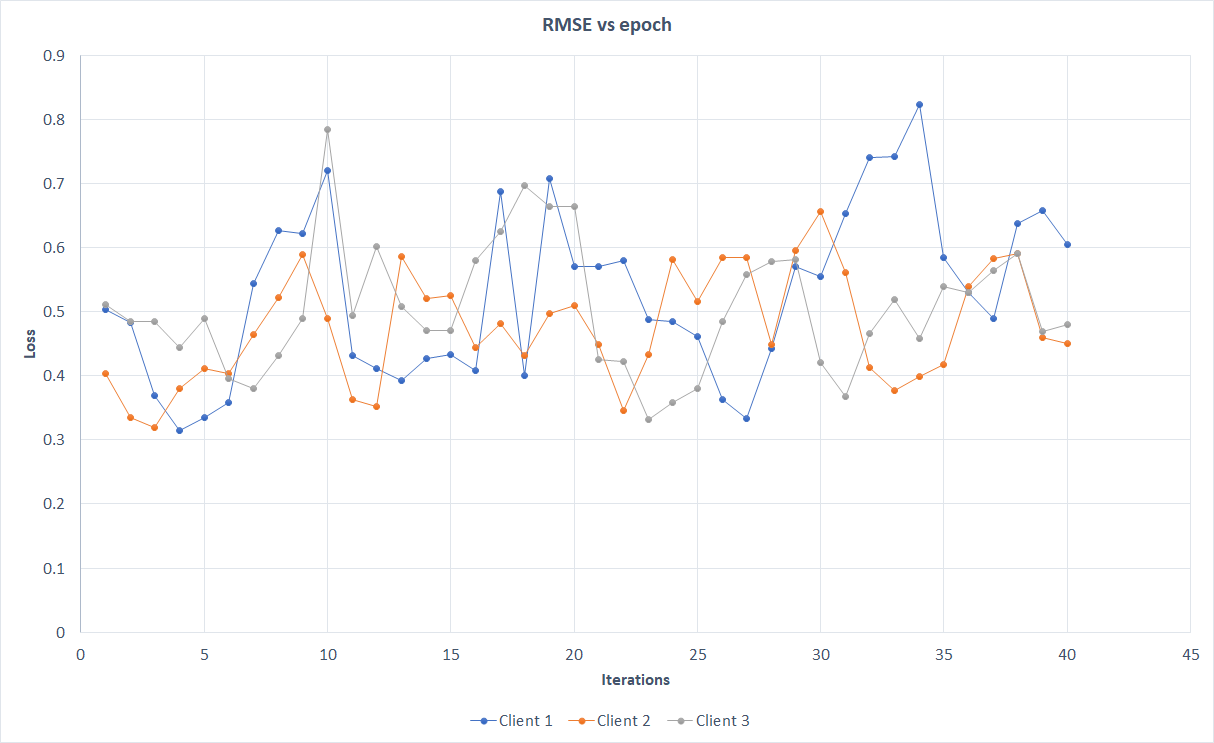
\includegraphics[width=90mm,scale=0.7]{RMSE_Secret_Sharing.png}

\caption{ RMSE  values  variation  with  number  of  Iterations for three clients}
\end{figure}

As shown in the \textbf{figure 9}, we can see that there is a lot of variation in the RMSE curves as compared to the figure 7, it's not converging and not reaching to global optima. It's happening because of the precision value of the shared parameters which is 3 in case of secret sharing and weights are changing so fast as compared to simple neural network which causes high and low RMSE sometimes. And if we are taking the high precision it's time complexity is increasing as it has many steps i.e. generate shares, distribute shares, model aggregating and reconstructing the shares using Lagrange interpolation and it needs high computational power CPU which shows us a trade-off between the accuracy vs resources required.

% \end{figure}

\begin{figure}
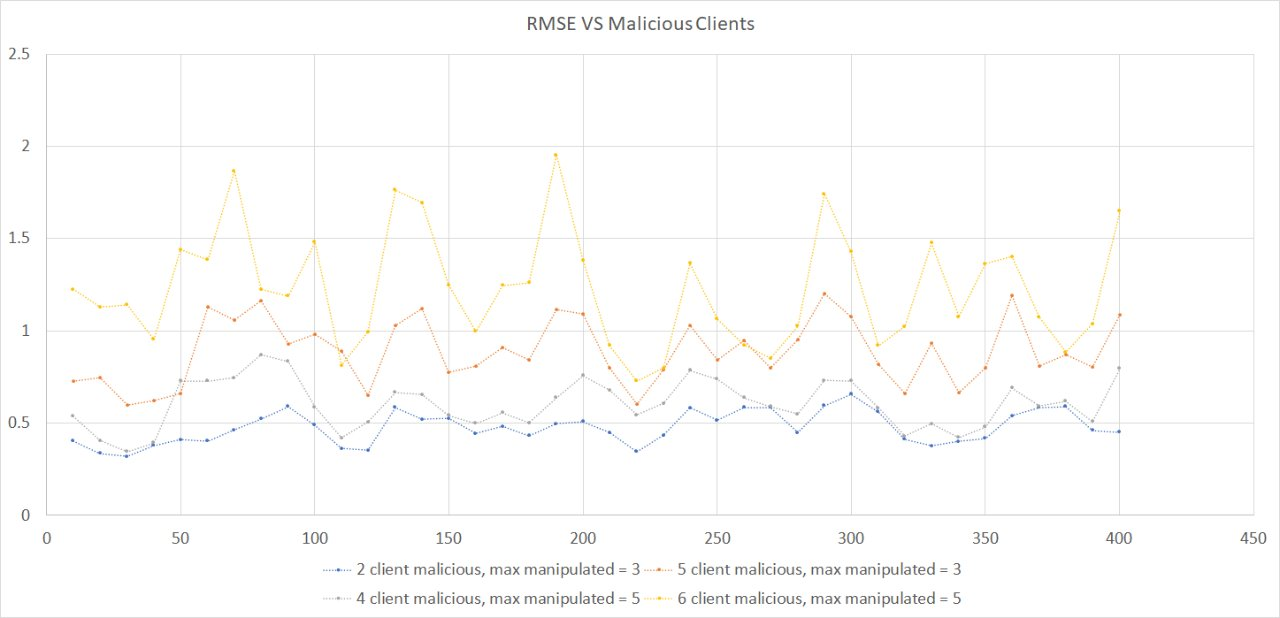
\includegraphics[width=90mm,height=70mm,scale=0.7]{RMSE_Malicious_SecretSharing.jpeg}

\caption{ RMSE  values  variation  with  number  of  Iterations for malicious clients}

\vspace{\baselineskip}

As shown in the \textbf{figure 10}, we can observe that there is a sudden bump or increase in the RMSE values curves as compared to the figure 1 when no. of malicious clients increases and no. of shares, max Failures are kept constant and max manipulated is N-K shares which means we need to have at least K shares to reconstruct the secret where N is the no. of shares generated and K is the no. of shares required to decrypt the secret. And we can successfully do an aggregation if we have atleast k shares at the server. 

\end{figure}

\begin{figure}

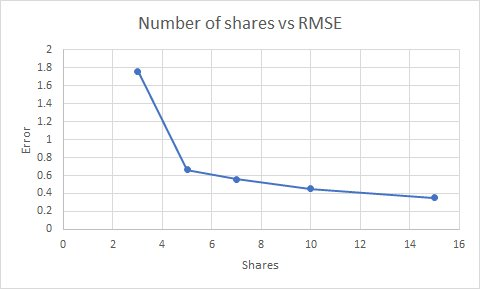
\includegraphics[width=90mm,scale=0.7]{numberofshares.jpeg}

\caption{ RMSE  variation  with  number  of shares used}

\vspace{\baselineskip}

As shown in the \textbf{figure 11}, the RMSE values are decreasing as the number of shares are increasing which is quite obvious because then each client will have a good mix-up of shares in this case and the malicious clients would not affect the model too much. But the computation time increases for the large number of shares and we need more powerful resources to prevent our model from malicious clients.

\end{figure}

\begin{figure}

\subsection{Comparison between the three protocols:}

\vspace{\baselineskip}

\textbf{RMSE Comparison:}

\vspace{\baselineskip}

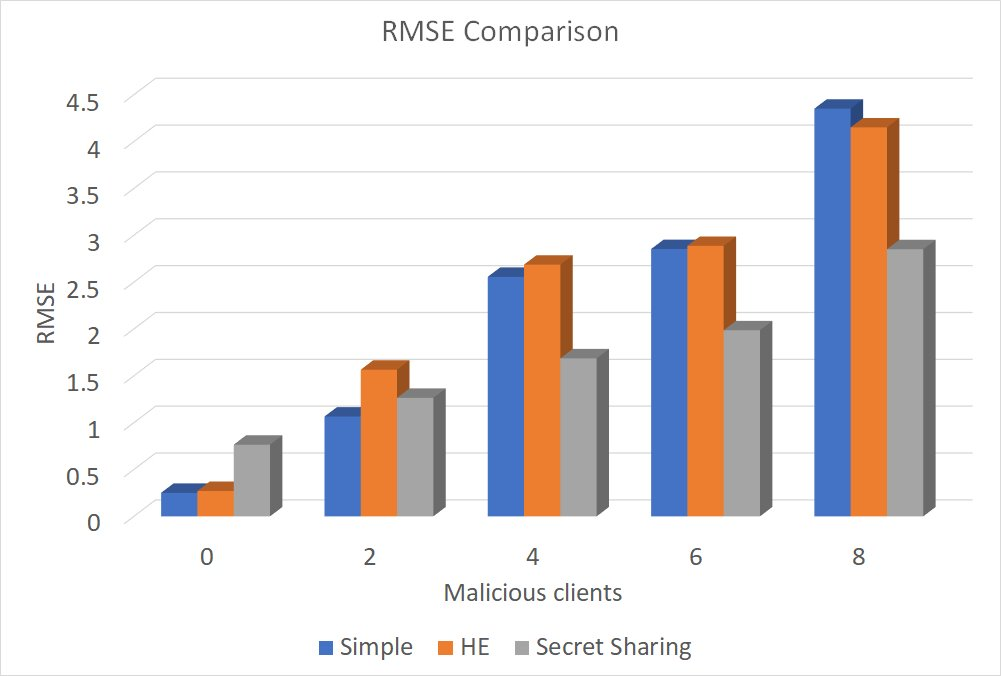
\includegraphics[width=90mm,height=80mm,scale=0.7]{secret_Simple_HE.jpeg}

\caption{ RMSE comparison for all 3 protocols}

\end{figure}

\begin{figure}

As shown in the \textbf{figure 12}, Initially with 0 or 2 malicious clients the Simple neural network and Homographic Encryption model is better than the secret sharing technique but it is performing worse if the no. of malicious clients are increasing which shows the secret sharing is better in a scenario where there are large number of malicious clients. It depends upon the situation of the environment from which we can decide the model one should go with.

\vspace{\baselineskip}

\textbf{Time Comparison:}

\vspace{\baselineskip}

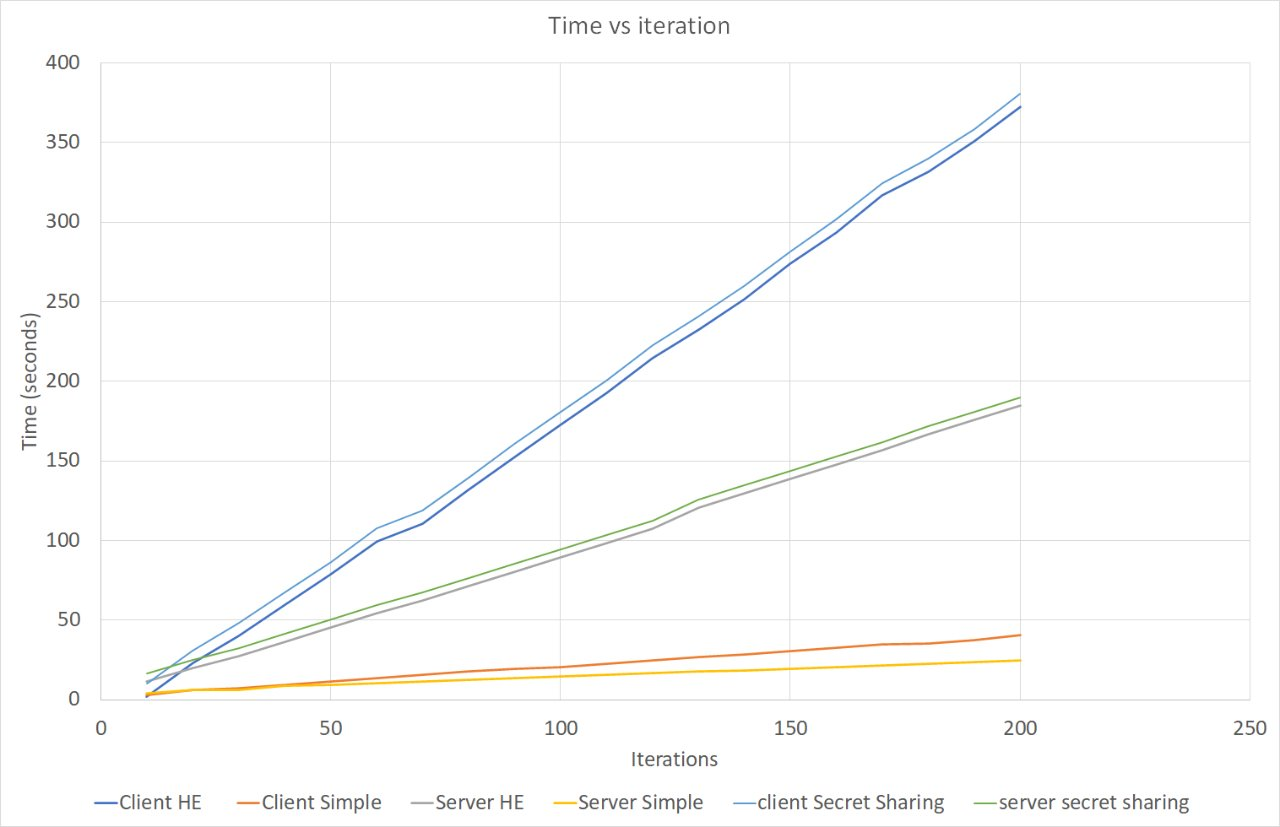
\includegraphics[width=90mm,scale=0.7]{all_time_comparison.jpeg}

\caption{ Wall-clock running time comparison for all 3 protocols}
\end{figure}
\begin{figure}

\textbf{ Data-overhead Size Comparison:}

\vspace{\baselineskip}

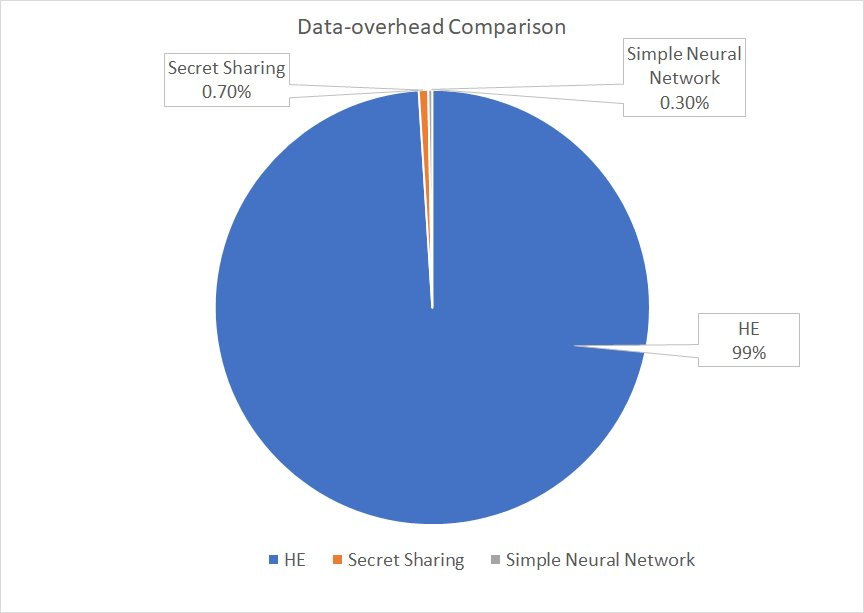
\includegraphics[width=90mm,scale=0.7]{Data_overhead_all.jpeg}

\caption{ Data-overhead comparison for all 3 protocols}

As shown in the \textbf{figure 13}, the time taken for each iteration by the client and server is almost same for Homographic Encryption and Secret Sharing though it's value is somewhat large for Secret Sharing technique. And the time consumed in case of simple neural network is small which shows the trade-off between the privacy and computation time.

\vspace{\baselineskip}

As shown in the \textbf{figure 14}, the size of data overhead is too much which is almost(100\%) for Homographic Encryption as compared to the other two. As each parameter is encrypted and encoded which has approximate 20000000 bytes(20 MB) length. On the other hand, the data overhead size is almost negligible in case of secret sharing and simple neural network.

\section{Conclusion}
In this report, we implemented a privacy-preserving federated learning scheme using different cryptographic algorithms i.e. Homographic Encryption and Secret Sharing. We also discussed the privacy related issues and threats to model in a general federated learning approach and tried to use the homographic encryption and secret sharing techniques, which can force the central server to conduct the aggregation operation, and is robust against user dropouts and malicious users. Then, using the designed secure aggregation scheme, we designed a suite of secure protocols to implemented the distributed Neural network linear regression model. Comprehensive experiments were conducted to evaluate the effectiveness and efficiency of both the approaches. Experiment results showed that \textbf{Secret Sharing} made it possible to train the neural network in the malicious and manipulated environment with some performance loss, and attained computation and communication cost reduction for secure aggregation. However, Homographic encryption and general approach couldn't handle the user dropouts and manipulated users but showing some good and accurate results in terms of performance and the data-overhead of communication was too large in case of Homographic Encryption. 

\section{Future Work}

We have looked at both the cryptography algorithms in which \textbf{secret sharing} was showing some promising results in terms of privacy. But we actually need to improve the performance of the system and try to reduce the loss and time complexity 

% <OR> manually copy in the resultant .bbl file
% set second argument of \begin to the number of references
% (used to reserve space for the reference number labels box)

% that's all folks

\end{figure}

by following ways:-

\begin{enumerate}
    \item Various approaches for reconstructing the secret i.e. Fast Fourier Transform and Newton's method which can improve the time complexity and hence precision. 
    \item Scaling and designing of the distributed systems for large number of clients
    \item Design a System with mixed approach of Homographic Encryption and Secret Sharing
    \item Reach to \textbf{Serverless} architecture by removing central authority
    \item Checking beats of all the instances using multi-threading
\end{enumerate}

\begin{thebibliography}{1}

\bibitem {cantrell1}
Ronald L. Rivest, ``Cryptography and machine learning'' \emph{Supported by NSF grant CCR-8914428, ARO grant N00014-89-J-1988, and the Siemens Corporation}

\bibitem {cantrell2}
Runhua Xu, Nathalie Baracaldo, Yi Zhou, Ali Anwar and Heiko Ludwig``HybridAlpha: An Efficient Approach for Privacy-Preserving Federated Learning'', \emph {ACM ISBN 978-1-4503-6833-9/19/11. . .}

\bibitem {krauss}
H. Brendan McMahan, Eider Moore, Daniel Ramage, Seth Hampson, Blaise Aguera y Arcas \emph{"Communication-Efficient Learning of Deep Networks from Decentralized Data"}, Google, Inc., 651 N 34th St., Seattle, WA 98103 USA

\bibitem {krauss}
Brendan McMahan and Daniel Ramage "Federated Learning: Collaborative Machine Learning without Centralized Training Data", \url{https://ai.googleblog.com/2017/04/federated-learning-collaborative.html} Google, Inc., 651 N 34th St., Seattle, WA 98103 USA

\bibitem {krauss}
Qinbin Li, Zeyi Wen, Zhaomin Wu, Sixu Hu, Naibo Wang, Bingsheng He, "A Survey on Federated Learning Systems: Vision, Hype and Reality for Data Privacy and Protection", \emph{arXiv:1907.09693v4 [cs.LG] 1 Apr 2020}

\bibitem {krauss}
Michele Minelli, "Fully homomorphic encryption for machine learning", "Cryptography and Security
[cs.CR]"  \emph{Université Paris sciences et lettres, 2018. English. ffNNT : 2018PSLEE056ff. fftel-01918263v2f}

\bibitem {krauss}
Lidong Zhou, "Secret Sharing", CS Cornell, USA
\url{http://www.cs.cornell.edu/courses/cs513/2000SP/SecretSharing.html}

\bibitem {krauss}
Maeva Benoit and Morten Dahl, "How Practical is Somewhat Homomorphic Encryption Today?", \url{https://medium.com/snips-ai/how-practical-is-somewhat-homomorphic-encryption-today-6818d1c6f7f6}

\bibitem {krauss}
Morten Dahl, "High-Volume Secret Sharing"
\url{https://medium.com/snips-ai/optimizing-threshold-secret-sharing-c877901231e5}

\bibitem {krauss}
Yang Liu Zhuo Ma, Ximeng Liu, Siqi Ma, Surya Nepal, Robert.H Deng, Kui Ren, "Boosting Privately: Federated Extreme Gradient Boosting for Mobile Crowdsensing" \emph{arXiv:1907.10218v2 [cs.CR] 10 Apr 2020}

\bibitem {krauss}
Secret double octopus, "The Secret Security Wiki"
\url{https://doubleoctopus.com/security-wiki/encryption-and-cryptography/secret-sharing/}

\bibitem {krauss}
Wikipedia the free encyclopedia, "Lagrange polynomial"
\url{https://en.wikipedia.org/wiki/Lagrange_polynomial}

\bibitem {krauss}
Chuan Ma , Jun Li, Ming Ding, Howard H. Yang, Feng Shu, Tony Q. S. Quek, H. Vincent Poor "On Safeguarding Privacy and Security in the Framework of Federated Learning"
\emph{arXiv:1909.06512 [cs.NI]}

\bibitem {krauss}
Ahmed Gad "Breaking Privacy in Federated Learning"
\url{https://heartbeat.fritz.ai/breaking-privacy-in-federated-learning-77fa08ccac9a}

\bibitem {krauss}
Jonas Geiping, Hartmut Bauermeister, Hannah Dröge, Michael Moeller, "Inverting Gradients -- How easy is it to break privacy in federated learning?" \emph{arXiv:2003.14053 [cs.CV]}

\bibitem {krauss}
Daniel Huynh, "Homomorphic Encryption intro: Part 1: Overview and use cases"
\url{https://towardsdatascience.com/homomorphic-encryption-intro-part-1-overview-and-use-cases-a601adcff06c}

\bibitem {krauss}
Keith Bonawitz, Vladimir Ivanov, Ben Kreuter, Antonio Marcedone†‡,H. Brendan McMahan, Sarvar Patel, Daniel Ramage, Aaron Segal and Karn Seth, "Practical Secure Aggregation for Privacy-Preserving Machine Learning" \emph{Cornell Tech, 2 West Loop Rd., New York, NY 10044}

%\bibitem{IEEEhowto:kopka}
%H.~Kopka and P.~W. Daly, \emph{A Guide to {\LaTeX}}, 3rd~ed.\hskip 1em plus
% 0.5em minus 0.4em\relax Harlow, England: Addison-Wesley, 1999.

%\bibitem{lamport} L. Lamport, \emph{ {\LaTeX} A Document Preparation
%  System}, Reading, Mass: Addison-Wesley, 1994.

%\bibitem{knuth} D. E. Knuth, \emph {The \TeX book}, Reading, Mass.:
%  Addison-Wesley, 1996.

\end{thebibliography}
\smallskip

\end{document}